\documentclass[11pt,a4paper]{article}
\usepackage{cite,url,hyperref,graphicx, amsmath, bm}
\usepackage{alltt} 
\usepackage{listings}
\usepackage{algorithm2e} % need texlive-science which I'm having trouble with getting...
\lstset{
basicstyle=\small\ttfamily,
columns=flexible,
breaklines=true
}



\setlength{\textwidth}{6.5in}
\setlength{\oddsidemargin}{0in}
\setlength{\evensidemargin}{0in}
\setlength{\topmargin}{-0.5in}
\setlength{\textheight}{25cm}
%opening
\title{Error Analysis of PSMC'}
\author{Alex Lee Jackson}
\begin{document}

\maketitle

%\begin{abstract}
%blah
%
%\end{abstract}
\section{Miscellaneous}
For further inquiries, I can be contacted at \href{mailto:aj123@internode.on.net}{aj123@internode.on.net}, or DM'd on the \texttt{rstat} Slack.

GitHub: \url{https://github.com/alex-jackson1994/errorAnalysis}

\section{Objective}
Determine if there's a relationship between the lengths of contigs being analysed, population model (predictors) and the error (response) given by PSMC' (MSMC\cite{schiffels2014inferring} with two haplotypes). This will probably be done using mixed effects models.\\

\begin{algorithm}[H]
  \For{Each population model (3)}{
    \For{Each simulated genome (5)}{
      \For{Each model of fragmentation (2)}{
        \For{Each level of fragmentation (5)}{
          Run MSMC, record output.\
        }
      }
    }
  }
  \caption{Outline of the simulation and MSMC analysis process}\label{overall}
\end{algorithm}

\subsection{Background}
PSMC' gives an estimate of how population demographics change over time, by analysing heterozygousity of sites across a genome. However, real sequenced genomes will not always be nicely sorted into chromosomes. Often they will be assembled into smaller sections called contigs. We will simulate human genomes (MSMC was originally written to analyse humans) under the following conditions:
\begin{itemize}
\item The length $L$ of the genome will be taken from a real human genome. For simplicity, \emph{only autosomes} will be considered.
\item Three different population models will be considered. Take time $t$ as going from recent to ancient, i.e. $t=0$ is the more recent than $t=100$. These dynamics should be carefully considered, as we want them to fall into the time range where PSMC' can actually pick them up.
\begin{itemize}
\item Constant: $N_e(t)=N_0$.
\item Exponential decrease: $N_e(t)=N_0e^{kt}$ for some realistic $k<0$.
\item Bottleneck: $N_e(t)=?$
\end{itemize}
\end{itemize}

%\begin{algorithmic}
%\State Set $L$.
%\For{<text>}
%<body>
%\EndFor
%\end{algorithmic}


\subsection{Potential Whole Genome Simulators}
We want a simulator with the following properties.
\begin{itemize}
\item Able to simulate exponential growth.
\item Able to be converted to a format which can be taken by MSMC.
\item Able to simulate linkage disequilibrium.
\item Uses the coalescent model, not forward model.
\item Can handle human genome sizes (in the range of 2.6 Gbp).
\end{itemize}
A number of simulators were considered.
\begin{itemize}
\item msHot-LITE (\url{https://github.com/lh3/foreign/tree/master/msHOT-lite}): This was used by Heng Li in his PSMC paper to simulate genomes. However, it has an upper size limit of roughly 10 Mbp.
\item GENOME (\url{http://csg.sph.umich.edu//liang/genome/}): This doesn't appear to do exponential growth.
\item GenomePop2 (\url{http://acraaj.webs.uvigo.es/GenomePop2.htm}): This can apparently output in ms-like format. Might go back to it later...
\item MaCS (\url{https://github.com/gchen98/macs}): Looking at this right now. It CAN handle the 2.6 Gbp sizes needed, as well as the other things I believe. Also, it's very fast.
\item scrm (\url{http://scrm.github.io/}): Recommended by Schiffels, but I haven't looked at it.
\end{itemize}

\subsubsection{MaCS}
\textbf{UNITS!!!}

For full detail, please refer to the MaCS README (\url{https://github.com/gchen98/macs/blob/master/README}), and the manual (\url{http://home.uchicago.edu/rhudson1/source/mksamples/msdir/msdoc.pdf}) for ms\cite{hudson2002generating}, from which MaCS is based upon. The MaCS README is fairly sparse, so I'd advise familiarising yourself with the relevant parts of the ms manual.

The MaCS README contains two examples of running MaCS. I'd advise taking the random seed, which is included in \texttt{stderr}, and storing it from each run. Alternatively, you could just specify the seed and store that each time. Reproducibility is important.

Further information can be found by running \texttt{./macs}. Note that:
\begin{itemize}
\item \texttt{<samplesize>} should always be 2, as we are simulating a diploid genome.
\item \texttt{<region in base pairs>} would be of the order of 2.6 Gbp. You should get this exactly from an empirical genome.
\end{itemize}
Switches of interest are: \texttt{-s} (sets seed), \texttt{-t} (sets mutation rate), \texttt{-r} (sets recombination rate), \texttt{-T} (outputs in a format that can be converted to the ms format), \texttt{-eG} (sets growth rate), and \texttt{-eN} (sets population size, sets growth rate to 0).

MaCS output should be able to be converted into the ms format via the included script \texttt{msformatter}. I've run this without errors, but haven't confirmed the ms format can then be converted to MSMC input format.

To convert from ms format to MSMC input format, use the script \texttt{ms2multihetsep.py}, included in the GitHub \url{https://github.com/stschiff/msmc-tools}. I haven't tried to use this yet.

\subsection{Simulation Parameters}
We will need the following parameters for the simulation.
\begin{itemize}
\item Genome size: obtaining this from an empirical human genome would be ideal. Remember, we are only considering autosomes.
\item Mutation rate: Julien suggests $1.25\times 10^{-8}$ mutations per bp per generation is the current best estimate. 
\item Recombination rate: I don't know a good estimate.
\item Population models (this defines $N_0$ as well). We originally had Julien give us suggestions for times/effective sizes for a constant-bottleneck model. However, I suggest you guys all sit down and figure out exactly where you would like past demographic events to happen (as we want to make sure MSMC can pick them up).
\end{itemize}
Apart from the ``chromosome-level'' of fragmentation, fragmentation models will have to be discussed. This includes finding a relevant empirical contig distribution, and some mathematical model for chromosomal fragmentation. Then you'll have to decide whether to do the fragmentation on the MaCS output, ms format, or the MSMC input.

\subsection{File Names And Data Frames}
This is up to you, but when we did the (unsuccessful) PSMC analysis we used the file names to store information about the simulation parameters. For example, say we had a MSMC output file corresponding to population demographic ``Constant'', simulated genome 2, fragmentation model ``Empirical'', and fragmentation level ``3''. Then the output file would be called something like \texttt{Constant\_2\_Empirical\_3.txt}. We could then use regular expressions in R to extract ``Constant'' etc. for storing in a data frame.

See Table \ref{df} for an example of data frame we could use for storing results.
\begin{table}[h]
	\caption{Example data frame for storing analysis results}
	\begin{center}
		\begin{tabular}{ccccc}
			\hline
			\textbf{Pop. Dem.} & \textbf{Sim. Number} & \textbf{Frag. Model} & \textbf{Frag. Level} & \textbf{Error} \\
                        \hline
                        Constant & 1 & Empirical & 1 & 2303 \\
                        Constant & 1 & Empirical & 2 & 4054 \\
                        \vdots & \vdots & \vdots & \vdots & \vdots \\
                        ExpDecr & 5 & Poisson & 5 & 1406 \\ \hline
		\end{tabular}
	\end{center} \label{df}
\end{table}


\subsection{Error Analysis}

\subsubsection{Definition Of Error}
We define the \emph{error rate} $\Delta (s_1,s_2)$ between two functions $s_1(t)$ and $s_2(t)$ as 
\begin{eqnarray}
\Delta (s_1,s_2) = \int_{t_R}^{t_A} |s_1(t)-s_2(t)| \,dt, \label{errorRate}
\end{eqnarray}
for sensible limits of integration $t_R$ (recent) and $t_A$ (ancient). Treat recent time as time near 0, and ancient time as time near $\infty$. The interpretation of this is the absolute value of the area between the two curves, in the interval $(t_R,t_A)$. Consult with Ben on choosing these values - a suggestion was the 95\% confidence interval for the time of coalescence between two haplotypes.

Is error going to be evaluated on a log scale?

Are you going to compare to the ``truth'' (simulation parameters), or to the ``best you can do'' (what MSMC recovers from the chromosomal level of fragmentation)?

\subsubsection{Calculating Errors}
Over the 2015/16 summer, the main script we used for calculating errors in PSMC was the following.
\begin{lstlisting}
~/Dropbox/MAGenomics_2015/PSMC_Scholarship/alexScripts/PSMC_Regression/StringExtraction_ErrorAnalysis.R
\end{lstlisting}
While this is optimised for the specific task we were doing, parts of it could be adapted for a MSMC analysis.

The main two functions of interest in the script are \texttt{eval\_popsize} and \texttt{absdifference}.

The function \texttt{eval\_popsize(pos, x, y)} takes a set of discrete points e.g. 
\begin{eqnarray*}
\{(t_1, N_{e}(t_1)), (t_2, N_{e}(t_2)), \cdots,(t_n, N_{e}(t_n))\}
\end{eqnarray*}
where \texttt{x} is a vector of $\{t_i\}$ and \texttt{y} is a vector of $\{N_e(t_i)\}$. Given a time point \texttt{pos}, the function will return the corresponding population size, if the $\{(t_i,N_e(t_i)) \}$ were connected by a step function. This allows us to construct the stepwise constant functions we see when MSMC graphs are plotted (see Figure \ref{pointsToStep}).

\begin{figure}
\centering
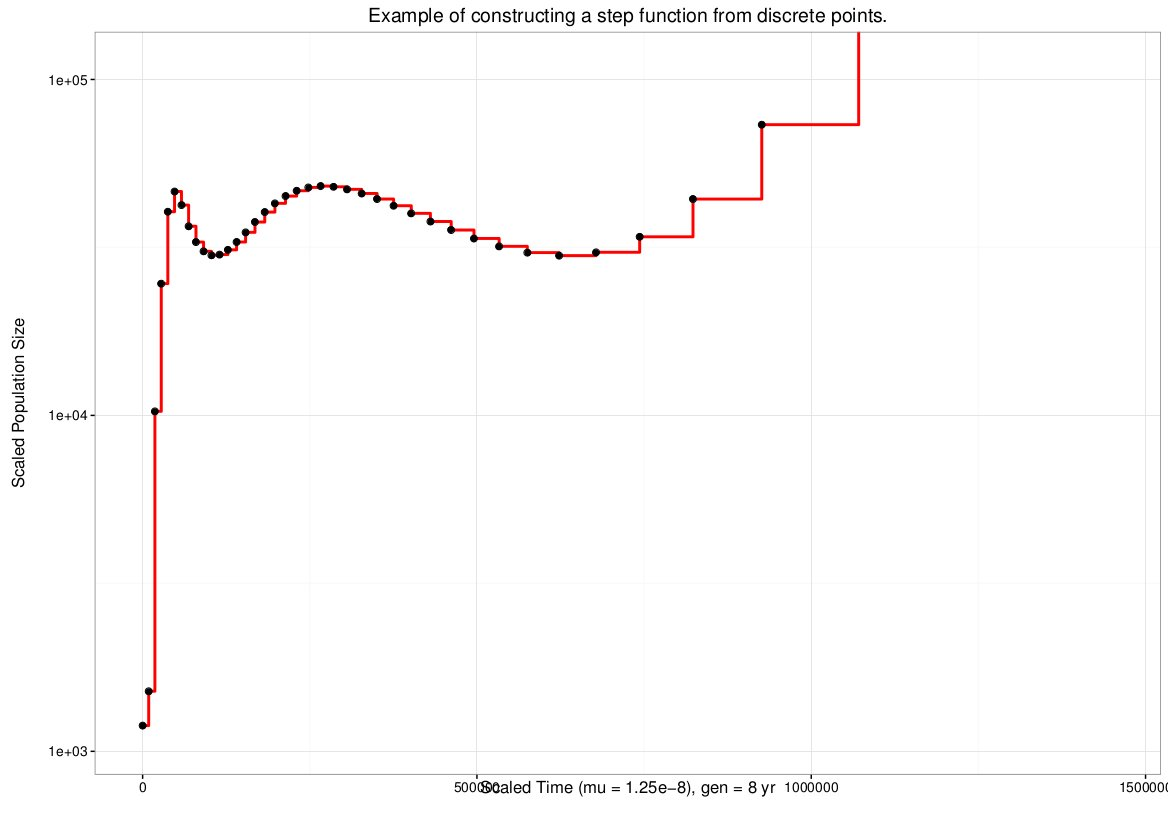
\includegraphics[width=1\textwidth]{pix/pointsToStep}
\caption{The function \texttt{eval\_popsize} allows us to construct a step function (red) from discrete points (black).} \label{pointsToStep}
\end{figure}

The function \texttt{absdifference(xpos,d1,d2,d3,d4)} returns the absolute difference between two MSMC stepwise constant functions $A$ and $B$, evaluated at point \texttt{xpos}. The other inputs to this function are \texttt{d1} and \texttt{d2} (vectors of $\{t_i\}$ and $\{N_e(t_i)\}$ respectively, for $A$), and \texttt{d3} and \texttt{d4} (vectors of $\{t_i\}$ and $\{N_e(t_i)\}$ respectively, for $B$). \texttt{absdifference} uses the \texttt{eval\_popsize} function.

One could then use R's integration function on \texttt{absdifference} to compute the integral that defines the error rate (Equation \ref{errorRate}).

Note that if you want to compare a ``true''  population model that involves curves (e.g. exponential growth) to MSMC output, the \texttt{absdifference} function may not be so useful. It might be better to write a new \texttt{absdifference} function which takes a MSMC stepwise constant function $A$ as one input, and a curve function $B$ as the other. However, this will be fine if comparing two MSMC curves (e.g. comparing the ``gold standard'' chromosomal fragmentation, with a much more fragmented genome).

\subsection{Running MSMC}
\subsubsection{Theory}

\textbf{Running MSMC. Link Graham the paper. Highlight the relevant parts, e.g difference from PSMC re: recombination rate estimates, time intervals. }

MSMC splits time from 0 (recent) to $\infty$ (ancient) into discrete unit time intervals. It then makes an estimate of population in each time interval. It then makes an estimate of the effective population in each interval (based on the heterozygousity of the genome).

The intervals are determined using the formula
\begin{eqnarray}
  t_i = \frac{-\ln (1-\frac{i}{n})}{{M\choose 2}} \label{timeInts}
\end{eqnarray}
for $i = 0, 1, \dots, n$. Here, $t_i$ is the time boundary of the particular interval, $n$ is the number of intervals (which you can define when running \texttt{msmc}, and $M$ is the number of haplotypes. As we will be looking at diploid individuals, the formula reduces to $t_i = -\ln (1-\frac{i}{n})$.

The unit intervals can be combined. For example, if you were running MSMC using the command 
\begin{lstlisting}
msmc -p 30*1 [...]
\end{lstlisting}
then this would be instructing the program to use 30 unit intervals ($n = 30$). If you used 
\begin{lstlisting}
msmc -p 10*1+15*2 [...]
\end{lstlisting}
then the program would use 10 unit intervals followed by 15 double-unit intervals ($n = 40$) (this also happens to be the defaults pattern). The left of \texttt{10*1+15*2} corresponds to recent time and the right corresponds to ancient time and the right corresponds to ancient time.

In the MSMC and PSMC papers, I have not found any justification for the use of particular combinations of time intervals.

I have found that if you scale MSMC time output such as in \texttt{plotMSMC\_PSMC.R}, you will \emph{not} get the same times as you do when you rescale the numbers you take from Equation \ref{timeInts}. To get the same times, you need to rescale by MSMC's estimate of mutation rate (which you should be able to find as \texttt{mutationRate} in the \texttt{log} file outputted by MSMC).

If you are interested, the recombination rate estimate \texttt{recombinationRate} can also be found in the \texttt{log} file.

\subsubsection{Using Real Data}
See attached example \texttt{runMSMC.txt}, which uses the Tasmanian Devil data. Julien should also be able to help with this. This will give a quick run-through of what the different commands are doing.

\begin{lstlisting}
awk '{print $1, 0, $2, $1, "0", "+"}' [...]
\end{lstlisting}
MSMC requires individual text input files per chromosome or contig. In this case, we look at the Devil \texttt{fasta} reference file to find the largest contigs to use. In this particular case, we only decided to use the contigs that were larger than 5 Mbp.

\begin{lstlisting}
module load python/4.8.0/3.4.1 gnu/4.9.2 zlib/testing samtools/1.2 bcftools/1.2 msmc/20150413 htslib/1.2.1 parallel
\end{lstlisting}
Load the relevant modules.

\begin{lstlisting}
parallel -j7 --nice 19 "samtools mpileup -EA -Q 20 -C 50 -u -r {} -f /localscratch/Refs/Sarcophilus_harrisii/Devil7_0_Raw [...]
\end{lstlisting}
You and Julien probably have a better idea of this than me. This creates the MSMC input files. For a different genome, obviously the names would have to be different. A \texttt{bam} genome and a \texttt{fasta} reference are required.

The next part is a copy from one of my files, 
\begin{lstlisting}
/localscratch/jsoubrier/Bison\_Genomes/CowRef/AlexPSMCMSMC\_Comparison/labBook
\end{lstlisting}
and should highlight relevant MSMC commands. Further information can be found on the GitHub guide (\url{https://github.com/stschiff/msmc/blob/master/guide.md}) or by running \texttt{msmc} on its own.
\begin{lstlisting}
msmc -t 50 -p 40*1 -i 20 -o EuropeanBison.Cow_UMD3_1.realigned_AllAutosomes_MSMCOutput EuropeanBison.Cow_UMD3_1.realigned_chr1_MSMCInput.txt EuropeanBison.Cow_UMD3_1.realigned_chr2_MSMCInput.txt [...] | at now
\end{lstlisting}
The switches of interest are: \texttt{-t} (sets number of threads to run on), \texttt{-p} (sets how MSMC divides up time from now to infinity in the past - more on that later), \texttt{-i} (number of iterations), and \texttt{-o} (set the name of the output file). The \texttt{--fixedRecombination} flag should be left out for running on two haplotypes (our situation), according to the guide.

Following the name of the output file are the MSMC input files (there were 29 in this case). This can make the commands long and messy. Finally, the \texttt{| at now} allowed me to leave this running on the server and then log off.

\subsubsection{Using Simulated Data}
I am not sure how to do this, but presumable it would go something like this:
\begin{enumerate}
\item Run MaCS (or similar) with the \texttt{-T} flag to output in the appropriate format.
\item Convert this to ms output format with the \texttt{msformatter} script which comes with MaCS.
\item Convert this to MSMC input format with \texttt{ms2multihetsep.py} included with Schiffels' MSMC tools.
\item (Fragment somewhere in here.)
\item Run MSMC as above.
\end{enumerate}

\subsection{Visualising MSMC}
See the attached example file \texttt{plotMSMC\_PSMC.R} for an annotated R file which runs through plotting MSMC (and PSMC). Just remove the parts relevant to PSMC if you only care about MSMC.


\section{Other Suggestions}
\subsection{Reduction In Complexity}
Julien suggested that we could do some trials to see if we recover the same dynamics with say 5 chromosomes, instead of the full 23. This would significantly decrease the run-time of the whole progress. However, fragmenting 5 chromosomes may be quite different to fragmenting 23 chromosomes.

\subsection{How To Use PSMC}
Should I include this?

\bibliographystyle{plain}
\bibliography{../references/references}{}


\end{document}
